\chapter{Focus Group} \label{chapter:focus-group}
As the previous usability study has shown, the naming of features was a major usability issue. Participants have been exposed to entirely new concepts. Errors that have been made during the sessions were often related to a misunderstanding of what a feature does. How things are phrased influences a user’s comprehension of a system, his or her mental model, strongly. As described in Chapter \ref{chapter:related-work} Git's conceptual model is flawed in certain ways, which is also reflected in its terminology. In order to avoid adopting these flaws for the content authoring tool, some Git concepts had to be revised, reconsidered or combined. This is why new names needed to be found for these concepts, which would properly reflect their purpose and help users to form an accurate mental model. The goal of the focus group was to identify those concepts that are particularly problematic as well as ideating on better names. The expected outcome were new ideas as well as valuable input for the second design iteration.

%In the tradition of co-operative design \cite{ehn_cooperative_2000} a workshop was held including the participants of the first usability study as well as the team working on the content authoring tool.

% talk a bit about co.design?

%write how this was also about identifying what the difficult terms are -> more focus on discovery and getting insights than on generating new ideas

%\section{Objectives}
%First and foremost the focus group is intended to provide a better understanding of the user’s thought process. Which terms are hard to understand or even misleading? Can they derive a function’s purpose based on its name? Since the participants were already exposed to the terms and corresponding features they will be able to provide feedback based on their own experience. Besides gaining insights the focus group also aims at producing suggestions for improvements. How can terms be rephrased to allow an easier understanding?

\section{Procedure}
The focus group was scheduled for 90 minutes with a short break in between. The first part consisted of an open discussion among the participants of the first usability study, during which they talked about their difficulties during the test sessions. They were briefed to put particular emphasis on the language used within the interface. In case the discussion steered off into another direction, the author, who acted as the facilitator, tried to direct it towards the terminology aspect again.

During the second phase, participants were expected to come up with alternatives for the current naming. In a short survey, prior to the meeting, participants had voted which features and terms they found most puzzling (See below). The results of the survey as well as the outcome of the previous usability study, formed the basis for the discussions during the second phase. In order to provide participants with a more solid understanding of version control, a short presentation was given before the start of the second phase. Afterwards participants were asked to conceive alternatives for the most problematic terms. At first for themselves and later on together with their peers.

\section{Most Problematic Terms}
In a short survey prior to the meeting participants had been asked how well they had understood different version control concepts. The 5 least understood terms or features were Pull Requests, Branches, Merging and the Reviewer functionality. Furthermore, the previous usability study has shown that naming of the default branch ("master branch", Issue \#4) and the history (Issue \#24) can cause problems as well.

\section{First Phase}
The first phase, the open discussion, showed that still a lot of confusion prevailed among the participants regarding the most common version control concepts. It is hard to say whether this is because of the names used for these concepts or because the concepts are inherently hard to understand. Branch and pull request, for example, seemed to be most problematic, but they are also conceptually the most complex. One of the participants even thought they are more or less the same thing. Another one mentioned, she could not tell the difference between the three concepts of unsaved changes, history and pull requests and had no idea in which order to use them. To conclude, one could say, that none of the participants (except for one) had formed an accurate mental model of the system, which is not surprising, given that they have only used it once and were not introduced to it before.

The participants agreed that it is easier to understand the concepts once they are explained, but they also stated that freelancers likely will not have this luxury. Most people agreed that illustrations, explanations and tooltips can be a great help while using the system.

% \begin{figure}[h!]
%  \centering
%  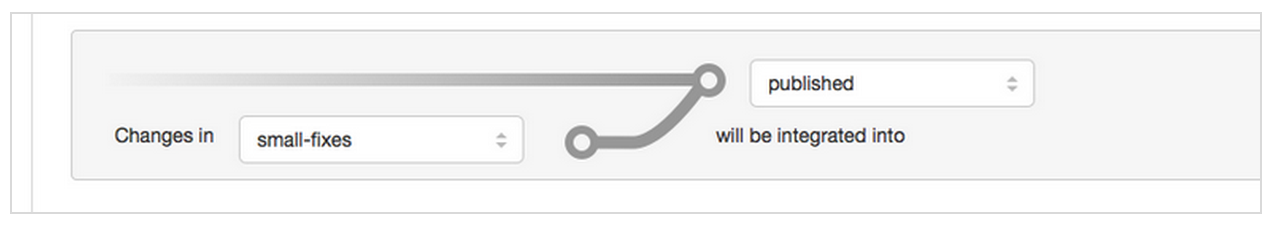
\includegraphics[width=\textwidth]{branch-visualization}
%  \caption{Illustration that visualizes what happens when two branches are merged}
%  \label{fig:branch-visualization}
% \end{figure}

\section{Second Phase}
At the beginning of the second phase the author gave a short introduction to version control and the most important concepts. This was done to provide the participants with a solid understanding of version control and its concepts, thus making it easier for them to come up with alternative names. The brainstorming proved to be more difficult than expected, but yielded a handful of alternative terms for each concept that had been deemed hard to comprehend earlier. What made it difficult to find different names for some concepts was the large domain they have to work for. For example, a translator creates a pull request in order to request proofreading, but one can not name it “request proofread”, because for some users it serves a different purpose. Some of the terms listed in Table \ref{table:alt-terminology} have a slight deficit in that they do not properly reflect the underlying concept. For example, “Publish Changes” will not work, because one can also merge changes into a branch that is not public (i.e. every branch except the master branch). Furthermore, “Request of Changes” sounds more like someone is requesting to change something and not like he or she has already changed something. Besides these negative examples, there are a couple of viable options that, after further consideration, could become part of the next prototype.

\begin{table}[h!]
\begin{tabular}{|l|l|l|}
\hline
\rowcolor[HTML]{EFEFEF}
{\bf Pull Request} & {\bf Merge (Pull Request)} & {\bf Branch}           \\ \hline
Check Changes      & Finalize                   & Working version        \\
Request of Changes & Publish Changes            & Experimental version   \\
Request Approval   & Accept Changes             & Copy                   \\
Request Review     & Approve Changes            & Draft                  \\
                   & Save                       & Public/Private Version \\
                   & Authorize                  &                        \\ \hline
\end{tabular}
\centering
\caption{Suggested alternative terms}
\label{table:alt-terminology}
\end{table}

\section{Conclusion}
The focus group has shown that it is almost impossible to detach a user’s understanding of a concept from its name. A weak mental model of a system can be the result of inconsistent concepts or bad names, or both. In this regard, the focus group did not help to illuminate this problem area. On the other hand, some viable alternatives to existing terms were found. The next design iteration, which is described in the next chapter, utilizes some ideas and the insights gained through this focus group. The subsequent usability study then evaluates whether a new naming scheme contributes to an improved usability.
